\section*{8 Flows on ABPs}
We now proceed to the analysis of $\g_0\fcom$ and $\g_0f_0$. The connection to flow vector spaces will be even more prevalent than in Proposition 12. The main result of this section is $\dim\g_0\fcom>\dim\g_0f_0$ (Theorems13 and14), which implies that $\fcom$ and $f_0$ have different orbit dimensions. We thereby conclude that $f_0\notin G\fcom$.
To each edge $e$ we assign its path tensor $\psi(e)$ by summing tensors over all valid paths passing through $e$,
\[\psi(e):=\sum_{\substack{p\in\mathcal P\text{ with }e\in p}}\varphi(p)\in E_1\otimes\cdots\otimes E_d.\]
By linear continuation this gives a linear map $\psi:\C^E\to E_1\otimes\cdots\otimes E_d$. Observe that $\psi(e)=A^{(i)}_{e,e}\fcom$. Let $T$ denote the linear span of all $\psi(e)$, $e\in E$. In other words, $T=\g_0\fcom$.
Let $\mathcal P'\subseteq\mathcal P\subseteq\mathcal X$ be the set of valid paths that contain exactly one parity preserving edge. To each edge $e$ we assign its parity path tensor $\psi'(e)$ by summing tensors over paths in $\mathcal P'$,
\[\psi'(e):=\sum_{\substack{p\in\mathcal P'\text{ with }e\in p}}\varphi(p)\in E_1\otimes\cdots\otimes E_d.\]
By linear continuation this gives a linear map $\psi':\C^E\to E_1\otimes\cdots\otimes E_d$. Observe that $\psi'(e)=A^{(i)}_{e,e}f_0$. Let $T'$ denote the linear span of all $\psi'(e)$, $e\in E$. In other words, $T'=\g_0f_0$.
We will establish the following bounds on the dimensions of $T$ and $T'$.
\begin{theorem}$\dim T=|E|-\sum_{i=1}^d w_i+1$.\end{theorem}
\begin{theorem}$\dim T'\le|E|-\sum_{i=1}^d w_i$.\end{theorem}
The rest of this section is dedicated to the proofs of Theorem 13 and Theorem 14 by showing that $T$ is isomorphic to the vector space of flows ``on the ABP'', while the parity constraints lead to a smaller dimension of $T'$.
From an ABP $\Gamma$ we construct a digraph $\widetilde\Gamma$ by identifying corresponding vertices from the first and the last layer in $V$ and calling the resulting vertex set $\widetilde V$. Note $|\widetilde V|=\sum_{i=1}^d w_i$. The directed graphs $\Gamma$ and $\widetilde\Gamma$ have the same edge set. The resulting directed graph is called $\widetilde\Gamma=(\widetilde V,E)$. Let $F$ denote the vector space of flows on $\widetilde\Gamma$. Note that by (11) we have $\dim F=|E|-|\widetilde V|+1$. All directed cycles in $\widetilde\Gamma$ have a length that is a multiple of $d$. In particular, all cycles of length exactly $d$ are in one-to-one correspondence with valid paths in $\Gcom$. For an edge $e\in E$, let $\chi(e)\in\C^E$ denote the characteristic function of $e$, i.e., the function whose value is1 on $e$ and0 everywhere else.
We now prove Theorem 13 by establishing a matching upper (Lemma 15) and lower bound (Lemma 16) of $|E|-|\widetilde V|+1=\dim F$ on $\dim T$.
\paragraph{The upper bound.}
\begin{lemma}$\dim T\le|E|-|\widetilde V|+1$.\end{lemma}
\begin{proof}
For $v\in\widetilde V$, let $\inset(v)\subseteq E$ denote the set of incoming edges incident to $v$ and $\outset(v)\subseteq E$ denote the set of outgoing edges incident to $v$. For each $v\in\widetilde V$, define the row vector
\[r_v=\sum_{e\in\inset(v)}\chi(e)-\sum_{e\in\outset(v)}\chi(e).\]
These vectors are the rows of the signed incidence matrix of $\widetilde\Gamma$, and since $\widetilde\Gamma$ is connected, they span a space of dimension $|\widetilde V|-1$ ([8, Ex.1.5.6]). Now observe that for all $v\in\widetilde V$,
\[\sum_{e\in\inset(v)}\psi(e)=\sum_{e\in\outset(v)}\psi(e).\]
Since $\psi$ is linear, this is equivalent to
\[\psi\left(\sum_{e\in\inset(v)}\chi(e)-\sum_{e\in\outset(v)}\chi(e)\right)=0.\]
Hence each $r_v$ is in the kernel of $\psi$, and hence $\dim\ker\psi\ge|\widetilde V|-1$. Using (11), we obtain
\[\dim T=\dim\im\psi=|E|-\dim\ker\psi\le|E|-|\widetilde V|+1=\dim F.\]
\end{proof}
\paragraph{The lower bound.}
To obtain the lower bound, we define a linear map $\varrho:E_1\otimes\cdots\otimes E_d\to\C^E$ such that the image of $\varrho$ restricted to $T$ equals $F$. This will imply that $\dim T\ge\dim F$, thereby achieving the required lower bound.
We define the linear map $\varrho$ on standard basis elements $x_{e_1}\otimes\cdots\otimes x_{e_d}$ as follows,
\[\varrho(x_{e_1}\otimes\cdots\otimes x_{e_d}):=\chi(e_1)+\cdots+\chi(e_d),\]
and then extend it to the domain $E_1\otimes\cdots\otimes E_d$ via linear continuation.
\begin{lemma}
Let $\varrho|_T$ denote the restriction of $\varrho$ to the linear subspace $T$. Then, $\im\varrho|_T=F$. In particular, $\dim T\ge\dim F=|E|-|\widetilde V|+1$.
\end{lemma}
\begin{proof}
To prove equality it suffices to show $\im\varrho|_T\subseteq F$ and $F\subseteq\im\varrho|_T$.
The first containment is easy to see. For an edge $e$, consider the image of $\psi(e)$ under the map $\varrho$,
\[\varrho(\psi(e))=\sum_{e\in p\in\mathcal P}\sum_{e'\in p}\chi(e').\]
Observe that for a path $p\in\mathcal P$, $\sum_{e'\in p}\chi(e')$ is a flow on $\widetilde\Gamma$ and hence it belongs to $F$. Thus, we have $\varrho(\psi(e))\in F$. Since $T$ is spanned by $\psi(e)$, for $e\in E$, we obtain that $\im\varrho|_T\subseteq F$.
To establish the second containment it suffices to show that the image of $T$ under the map $\varrho$ contains a basis of $F$. We identify a specific basis for $F$ in Claim 17 and prove that it is contained in $\im\varrho|_T$ in Claim 18 to complete the argument.
\end{proof}
We identify directed cycles with their characteristic flows, i.e., flows that have value 1 on the cycle's edges and0 everywhere else. We also identify directed cycles that use edges in any direction with their characteristic flow: the characteristic flow is defined to take the value 1 on an edge $e$ if $e$ is traversed in the direction of $e$, and value$-1$ on $e$ if $e$ is traversed against its direction.
From the theory of flows we know that for every (undirected) spanning tree $T$ of $\widetilde\Gamma$, the vector space $F\in\C^E$ has a basis given by the characteristic flows of cycles that only use edges from $T$ and exactly one additional edge (for example, see Theorem 20.8 in [8]). Thus, the cycle flows corresponding to the elements not in the spanning tree form a basis of $F$.
\begin{claim}$F$ is spanned by the set of directed cycles in $\widetilde\Gamma$ of length exactly $d$.\end{claim}
\begin{figure}[tbp]\centering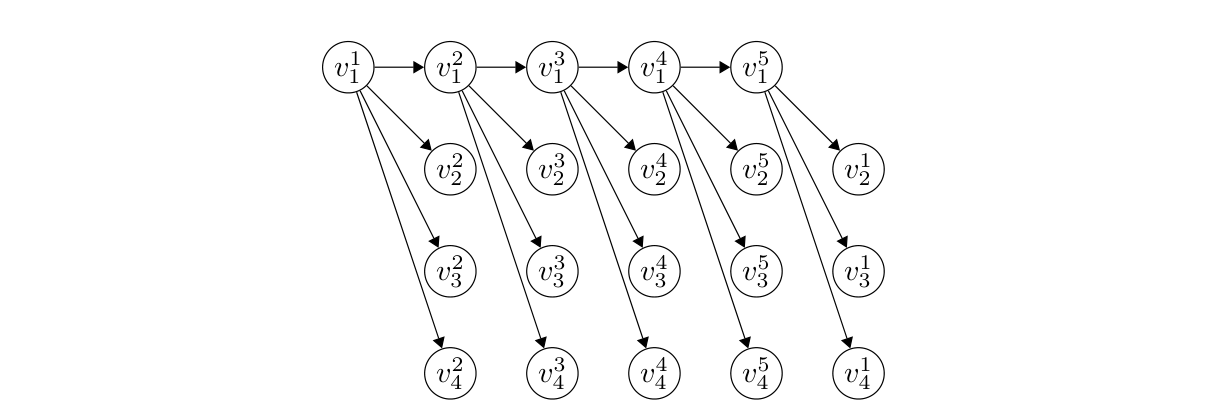
\includegraphics[width=\linewidth]{trace-fig1.png}\caption{The spanning tree construction for width 4 and $d=5$.}\end{figure}
\begin{figure}[tbp]\centering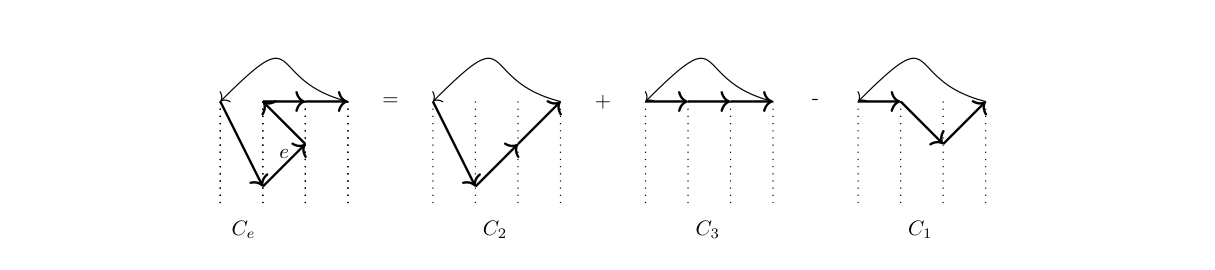
\includegraphics[width=\linewidth]{trace-fig2.png}\caption{Decomposing a cycle of length $d+2$ as a linear combination of cycles of length $d$. The figure is an illustration when $d=3$. The dotted layers in each cycle from the left are $V^3$, $V^1$, $V^2$, and $V^3$ again.}\end{figure}
\begin{proof}
We construct a spanning tree $\tau$ as follows, which will be a tree whose edges are all directed away from its root. Informally, the tree is given by the following subgraph, we make the first vertex in $V^1$ as root, and include all the outgoing edges incident to it. We then move to the first vertex in $V^2$ and include all the outgoing edges incident to it. We continue in this way until we reach $V^d$. Upon reaching the first vertex in $V^d$ we include all but one outgoing edges incident to it. The one that is an incoming edge to the root is not included. Figure 1 illustrates the construction. We now formally define this.
Let $v^i_1\in V^i$ denote the first vertex in the layer $i$, $1\le i\le d$. Further recall $\inset(v)\subseteq E$ and $\outset(v)\subseteq E$ denote the set of incoming and outgoing edges, respectively, incident to $v$. Define the edge set
\[\tau:=\left(\bigcup_{i=1}^d\outset(v^i_1)\right)\setminus\{(v^d_1,v^1_1)\},\]
which is a spanning tree in $\widetilde\Gamma$. We know that every edge not in the tree when added to the tree gives a unique undirected cycle. We now show that the characteristic flows of these undirected cycles can be expressed as a linear combination of the characteristic flows of directed cycles of length $d$. For $e\in E\setminus\tau$, let $c_e$ denote the characteristic flow of the unique undirected cycle that uses $e$ in its correct direction and only edges of $\tau$. We argue depending on which layer the edge $e$ belongs to.
\paragraph{Suppose $e\in E^1\setminus\tau$.}
\begin{itemize}
\item If $e$ is incident to $v^2_1$, the first vertex in $V^2$, then the inclusion of $e$ creates a directed cycle of length $d$. Hence, $c_e$ equals the characteristic flow of this directed cycle.
\item Otherwise, the inclusion of $e$ creates an undirected cycle of length $d+2$. If $e=(v^1_{j_1},v^2_{j_2})$ for some $j_1\in[2,w_1]$ and $j_2\in[2,w_2]$, then the cycle $c_e$ is given as follows:
\[v^d_1-v^1_{j_1}-v^2_{j_2}-v^1_1-v^2_1-\cdots-v^{d-1}_1-v^d_1.\]
Consider the following two directed cycles:
\begin{align*}C_1&:v^1_1-v^2_{j_2}-\cdots-v^d_1-v^1_1\text{ and}\\C_2&:v^1_{j_1}-v^2_{j_2}-\cdots-v^d_1-v^1_{j_1},\end{align*}
such that the part $v^2_{j_2}-\cdots-v^d_1$ between $v^2_{j_2}$ and $v^d_1$ in the two cycles is the same. Let us denote the characteristic flow of a cycle $C$ by $\chi(C)$. We now observe that $\chi(C_2)-\chi(C_1)$ equals the characteristic flow of the undirected cycle $v^1_{j_1}-v^2_{j_2}-v^1_1-v^d_1-v^1_{j_1}$. This is because the common part in $C_1$ and $C_2$ cancels out. To $\chi(C_2)-\chi(C_1)$ we add the characteristic flow of the directed cycle,
\[C_3:v^1_1-v^2_1-v^3_1-\cdots-v^{d-1}_1-v^d_1-v^1_1.\]
It is now easily seen that $\chi(C_2)-\chi(C_1)+\chi(C_3)$ equals the characteristic flow of the cycle $c_e$ (see Figure 2 for an illustration).
\end{itemize}
\paragraph{Suppose $e\in E^d\setminus\tau$.}
\begin{itemize}
\item If $e$ is incident to $v^1_1$, the first vertex in $V^1$, then as before the inclusion of $e$ creates a directed cycle of length $d$. Hence, $c_e$ equals the characteristic flow of this directed cycle.
\item Otherwise, the inclusion of $e$ creates an undirected cycle of length4. If $e=(v^d_{j_1},v^1_{j_2})$ for some $j_1\in[2,w_d]$ and $j_2\in[2,w_1]$, then the cycle $c_e$ is given as follows:
\[v^d_{j_1}-v^1_{j_2}-v^d_1-v^{d-1}_1-v^d_{j_1}.\]
Consider the following two directed cycles:
\begin{align*}C_4&:v^1_{j_2}-\cdots-v^{d-1}_1-v^d_1-v^1_{j_2}\text{ and}\\C_5&:v^1_{j_2}-\cdots-v^{d-1}_1-v^d_{j_1}-v^1_{j_2},\end{align*}
such that the part $v^1_{j_2}-\cdots-v^{d-1}_1$ between $v^1_{j_2}$ and $v^{d-1}_1$ in the two cycles is the same. We now claim that $\chi(C_5)-\chi(C_4)$ equals the characteristic flow of $c_e$. This is because the common part in $C_4$ and $C_5$ cancels out.
\end{itemize}
Otherwise $e\in E^i\setminus\tau$ for some $i\in\{2,\ldots,d-1\}$. In such a case inclusion of $e$ creates an undirected cycle of length4. We can again argue exactly like in the previous case, and so we omit the argument here.
\end{proof}
We now prove that the generating set given by the directed cycles of length $d$ is contained in the image of $T$ under the map $\varrho$.
\begin{claim}$\im(\varrho|_T)$ contains the characteristic flow of each directed cycle of length $d$.\end{claim}
\begin{proof}
Let $\{e_1,e_2,\ldots,e_d\}\subseteq E$ be a directed cycle of length $d$, where each $e_i$ points from a vertex in $V^i$ to a vertex in $V^{i+1}$. Let $\{e_i^{(j)}\}$ denote the set of edges that start at the same vertex as $e_i$, but for which $e_i^{(j)}\ne e_i$. Thus $|\{e_i^{(j)}\}|=|V^{i+1}|-1$. Let
\[\bar\psi(e):=\frac1{|\{p\in\mathcal P\text{ with }e\in p\}|}\psi(e),\]
so that $\varrho(\bar\psi(e))$ is a flow with value 1 on the edge $e$. It is instructive to have a look at the left side of Figure 3, where $\varrho(\bar\psi(e_1))$ is depicted. Subtracting $\frac1{w_3}\sum_{j=1}^{w_3-1}\varrho(\bar\psi(e_2^{(j)}))$ and adding $\frac{w_3-1}{w_3}\varrho(\bar\psi(e_2))$ reduces the support significantly and brings us one step closer to the cycle, see the right side of Figure 3. We iterate this process until only the cycle is left. Formally:
\begin{align*}
\chi(e_1,\ldots,e_d)={}&\varrho(\bar\psi(e_1))\\
&+\frac{w_3-1}{w_3}\varrho(\bar\psi(e_2))-\frac1{w_3}\sum_{j=1}^{w_3-1}\varrho(\bar\psi(e_2^{(j)}))\\
&+\cdots\\
&+\frac{w_d-1}{w_d}\varrho(\bar\psi(e_{d-1}))-\frac1{w_d}\sum_{j=1}^{w_d-1}\varrho(\bar\psi(e_{d-1}^{(j)})).
\end{align*}
\end{proof}
\begin{figure}[tbp]\centering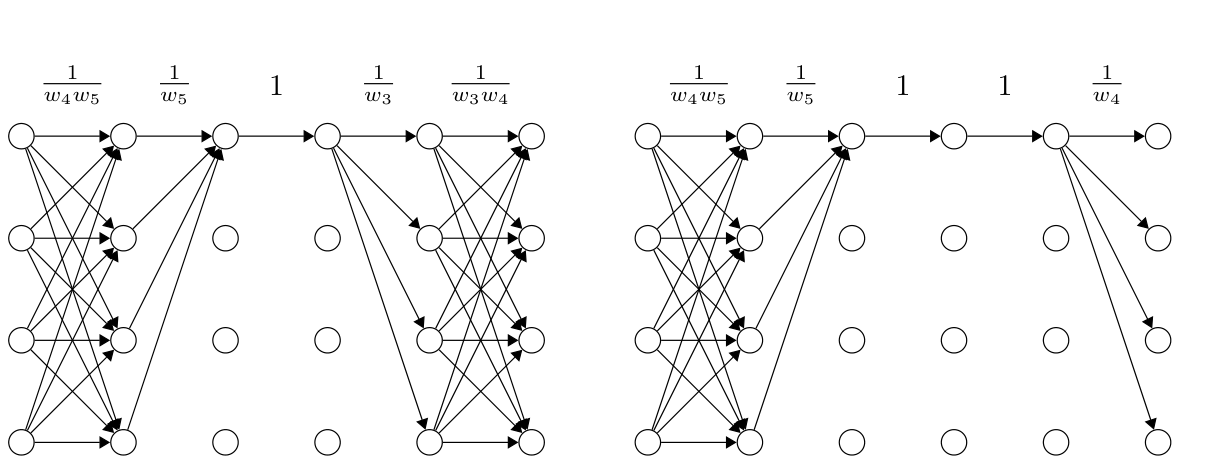
\includegraphics[width=\linewidth]{trace-fig3.png}\caption{On the left: $\varrho(\bar\psi(e_1))$. On the right: $\varrho(\bar\psi(e_1))-\frac1{w_3}\sum_{j=1}^{w_3-1}\varrho(\bar\psi(e_2^{(j)}))+\frac{w_3-1}{w_3}\varrho(\bar\psi(e_2))$. This is the case $d=5$ and format$(4,4,4,4,4)$. Edges that are not drawn carry 0 flow. All edges in the same layer carry either0 flow or the value that is depicted above the edge layer. For the purposes of illustation, $e_1$ is the top edge in the center. Here we assume that each $e_i$ points from the first vertex in $V^i$ to the first vertex in $V^{i+1}$.}\end{figure}
\paragraph{The stronger upper bound via parities.}
We now proceed to upper bound $\dim T'$ (Theorem 14). The proof is analogous to the proof of Lemma 15.
\begin{theorem}[Restatement of Theorem 14]$\dim T'\le|E|-|\widetilde V|$.\end{theorem}
\begin{proof}
As in the proof of Lemma 15, for $v\in\widetilde V$, we have
\[\sum_{e\in\inset(v)}\psi'(e)=\sum_{e\in\outset(v)}\psi'(e).\]
Furthermore, we have the following additional constraint on $\psi'$,
\[(d-1)\sum_{e\text{ parity preserving}}\psi'(e)=\sum_{e\text{ parity changing}}\psi'(e).\]
By the linearity of $\psi'$, we have
\[\psi'\left((d-1)\sum_{e\text{ parity preserving}}\chi(e)-\sum_{e\text{ parity changing}}\chi(e)\right)=0.\]
Therefore, the kernel of $\psi'$ is spanned by the vectors $(\sum_{e\in\inset(v)}\chi(e)-\sum_{e\in\outset(v)}\chi(e))$, for $v\in\widetilde V$, and an additional vector $((d-1)\sum_{e\text{ parity preserving}}\chi(e)-\sum_{e\text{ parity changing}}\chi(e))$.
We now claim that the new vector is linearly independent from the earlier set of vectors. We prove the claim by constructing a vector in $\C^E$ that is orthogonal to the earlier set of vectors but is non-orthogonal to the additional vector. One such vector is given by the characteristic flow of the directed cycle $v^1_1-v^2_1-v^3_1-\cdots-v^{d-1}_1-v^d_1-v^1_1$.
Thus, it follows that $\dim\ker\psi'\ge|\widetilde V|$, and hence $\dim T'\le|E|-|\widetilde V|$.
\end{proof}
